
\chapter{Introduction}

%=========================================================================

The study of the atmospheric general circulation is concerned with the dynamics of the climate system. It considers the time averaged characteristics of variables such as wind, temperature, humidity and precipitation, with the averaging applied over a period long enough to remove the random variations associated with individual weather systems, but short enough to retain monthly and seasonal variations. For a planet with a longitudinally uniform surface, the flow averaged over such a period would be the same at all points along a given latitude circle, since the average influence of zonally asymmetric transient eddies (i.e. weather disturbances) would be the same at all points. Large-scale topography and continent-ocean heating contrasts on Earth, however, provide strong forcing for zonally asymmetric planetary-scale motions in the monthly and seasonally averaged flow. These longitudinally dependent components of the general circulation may be categorised as quasi-stationary circulations, which vary relatively little in time (and are often referred to as stationary or planetary waves); monsoonal circulations, which are seasonally reversing; or various subseasonal and interannual components which together account for low-frequency variability \citep{Holton2013}. 

In the Southern Hemisphere (SH) extratropics, the primary zonal asymmetries are the quasi-stationary zonal wavenumber one (ZW1) and zonal wavenumber three (ZW3) circulations and a mode of low frequency variability known as the Pacific-South American (PSA) pattern. When superimposed on the zonal-mean circulation, the ZW1, ZW3 and PSA pattern produce local regions of enhanced and diminished time mean westerly winds, which strongly influence the development and propagation of transient weather disturbances. Persistent (or blocked) weather patterns, for instance, are typically associated with high-amplitude waves in the upper troposphere \citep[e.g.][]{Trenberth1985,Renwick2005}. These waveforms are also associated with the meridional transport of heat and moisture, which means variability in their amplitude and phase is associated with monthly and seasonal variations in variables such as temperature, precipitation and sea ice. Understanding the atmospheric drivers of climate variability in the mid-to-high southern latitudes has become an area of renewed interest recent years, in light of the rapid climatic changes observed in that region. Of particular relevance to the ZW1, ZW3 and PSA pattern is the fact that West Antarctica and the Antarctic Peninsula are among the most rapidly warming regions on Earth \citep[e.g.][]{Nicolas2014} and Antarctic sea ice has undergone a dramatic spatial redistribution \citep[e.g.][]{Simmonds2015}. 

Despite the fundamental role that the zonal waves and PSA pattern play in the SH general circulation (and perhaps recent high latitude trends), existing studies of their climatological characteristics are dated and somewhat limited in their scope. This chapter explores the details of our current climatological understanding, with particular focus on the wave identification methods used in relevant studies. The subsequent chapters go on to present updated climatologies that not only utilise a longer and higher quality dataset than previous studies, but that also develop and apply new wave identification methods. In an attempt to provide a practical solution to the reproducibility crisis in computational research, the results discussed in these chapters have been presented in a completely reproducible manner. It is proposed that the approach taken in documenting the computational aspects of the work could be adopted as a minimum communication standard by academic journals in the weather and climate sciences.

%========================

\section{The zonal waves}\label{s:zw_overview}

It was \citet{vanLoon1972} who first characterised SH planetary wave activity as the superposition of two zonally-oriented, quasi-stationary waveforms of wavenumber one and wavenumber three (e.g. Figure \ref{fig:zw_example}). Since that landmark study, the ZW1 and ZW3 patterns have been identified as dominant features of the mid-latitude circulation on daily \citep[e.g.][]{Kidson1988}, seasonal \citep[e.g.][]{Mo1985} and interannual \citep[e.g.][]{Karoly1989} timescales. Corresponding metrics and climatologies have been developed \citep{Raphael2004,Hobbs2007} and their relationship with circulation features including the Amundsen Sea Low \citep[ASL;][]{Turner2013} and two prominent quasi-stationary anticyclones in the sub-Antarctic western hemisphere \citep{Hobbs2010} have been investigated.

\begin{figure}
\begin{center}
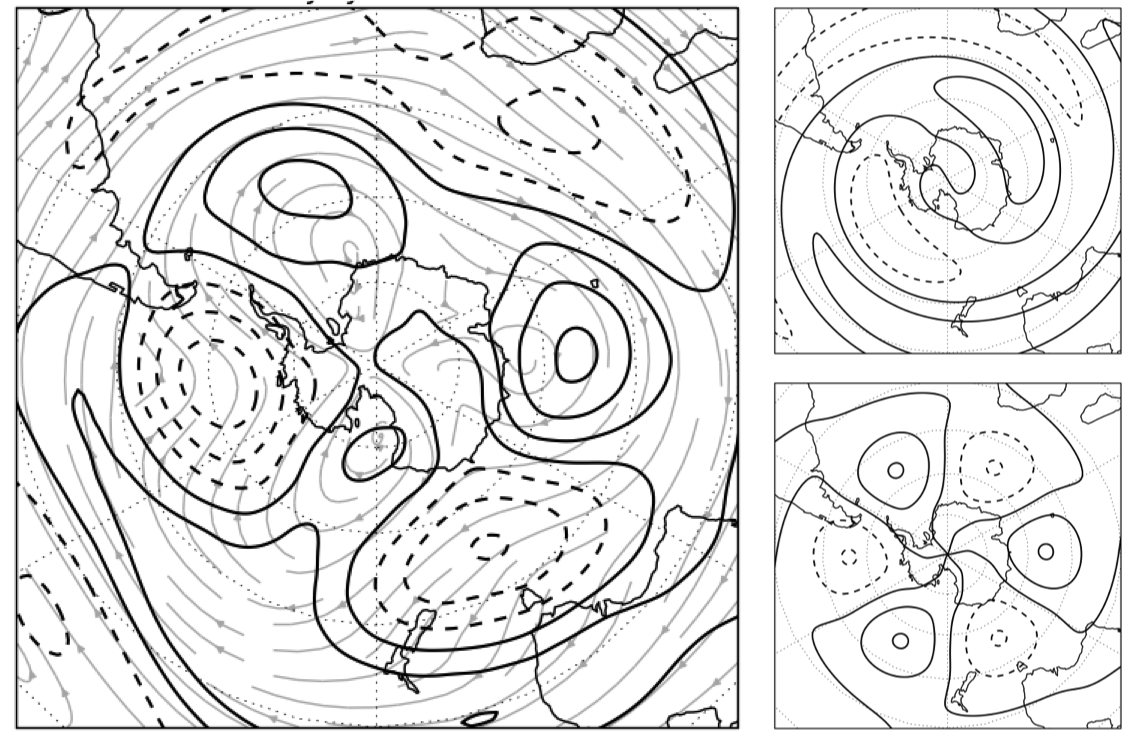
\includegraphics[width=0.7\columnwidth]{figures/zonalwaves/zw_example.png}
\caption[Mean 500 hPa circulation for July 2001 and the corresponding wavenumber one and three components of a Fourier transform]{\label{fig:zw_example}
Mean 500 hPa circulation for July 2001 (left) and the corresponding wavenumber one (top right) and three (bottom right) components of a Fourier transform. Grey streamlines indicate the direction of the wind, while the black contours show the streamfunction zonal anomaly (dashed contours indicate negative values and the contour interval is $5.0 \times 10^6 \: m^2 s^{-1}$).%
}
\end{center}
\end{figure}


While these climatologies and investigations reveal many of the basic characteristics of the ZW1 and ZW3 patterns (e.g. their variability and spatial pattern), with the exception of the ZW3 sea ice analyses of \citet{Raphael2007} and \citet{Yuan2008} and the ZW1 sea surface temperature (SST) results of \citet{Hobbs2007}, subsequent studies have not yet extended these climatologies to look at their influence on key variables such as surface air temperature and precipitation. Related studies on topics such as Australian \citep{Frederiksen2014} and Patagonian \citep{Garreaud2013} precipitation variability sometimes mention a ZW3-like pattern in passing, but the literature lacks a broad, hemispheric perspective on the link between planetary wave activity and regional climate variability. One reason for this might be that the ZW1 and ZW3 patterns never really occur in isolation, which makes analyses of just one or the other somewhat problematic \citep{Hobbs2010}.

In analysing the zonal waves, these previous studies have tended to define metrics based on either a stationary pattern or Fourier decomposition. With respect to the former, \citet{Raphael2004} defines a ZW3 index that is essentially the average 500 hPa geopotential height zonal anomaly across three key points (the annual average location of the ridges of the ZW3 pattern in the 500 hPa geopotential height field), while \citet{Yuan2008} use the principal component of the leading Empirical Orthogonal Function (EOF) mode of the surface monthly meridional wind. The stationary nature of these approaches means they cannot fully capture the subtle (approximately 15 degrees of longitude on average) seasonal migration in the phase of the ZW3 \citep{vanLoon1984,Mo1985} or the occurrence of patterns whose phase does not approximately coincide with the location of the three analysis points or leading EOF mode.

A number of studies have analysed the zonal waves by using a Fourier transform to express the upper tropospheric geopotential height in the frequency domain as opposed to the spatial domain \citep{Hobbs2007,Hobbs2010,Turner2013}. The output of a Fourier transform can be expressed in terms of a magnitude and phase for each wavenumber (or frequency/harmonic; the terminology differs in the literature), so these studies simply analysed the magnitude and phase information corresponding to the ZW1 and/or ZW3 pattern. While this might be considered an improvement on a grid point or EOF method in the sense that the phase is allowed to vary, a shortcoming is that the result is a constant amplitude wave over the entire longitudinal domain. The two major anticyclones associated with the ZW3 pattern (located over the western and eastern South Pacific respectively) are known to be positively covariant with respect to their location (indicating a coordinated wave pattern) but not amplitude \citep{Hobbs2010}, while in many cases ZW1- and/or ZW3-like variability is only prevalent over part of the hemisphere. As discussed in the seminal work of \citet{vanLoon1972}, it is clear that the other Fourier components (i.e. the non-wavenumber 1 or 3 coefficients) are required to modulate the amplitude of the ZW1 and ZW3 variability, and potentially vital information can be lost if those extra components are not incorporated when defining a metric of planetary wave activity. 

None of the aforementioned studies attempted to combine their ZW1 and ZW3 metrics to get a measure of total planetary wave activity, so for an example of this we must turn to the Northern Hemisphere (NH). In analysing the relationship between planetary wave activity and regional weather extremes, \citet{Screen2014} calculated the 500 hPa geopotential height Fourier amplitudes for a range of wavenumbers of interest, and then simply counted the number of positive and negative magnitude anomalies. While this may be an appropriate approach for the NH, it too fails to account for the fact that some of the waveforms in a Fourier transform simply exist to modulate others (something that was noted by \citet{Screen2014}) and thus it may not be appropriate to count all magnitude anomalies.


%========================

\section{The PSA pattern}\label{s:psa_overview}

First named by \citet{Mo1987}, the PSA pattern was identified in a number of studies of the large-scale SH circulation during the late 1980s and early 1990s \citep[e.g.][]{Kidson1988,Ghil1991,Lau1994}. A link between the pattern and Rossby wave dispersion associated with the El Ni\~{n}o-Southern Oscillation (ENSO) was soon found \citep[e.g.][]{Karoly1989}, and this work was followed by a number of detailed analyses of the characteristics of the pattern and its downstream impacts \citep[e.g.][]{Mo1998,Mo2000,Mo2001}.

The PSA pattern is most commonly analysed with respect to a pair of EOF modes (e.g. Figure \ref{fig:eof}). Known as PSA-1 and PSA-2, these modes are in quadrature and depict a wave train extending along an approximate great circle path from the central Pacific Ocean to the Amundsen and Weddell Seas. Some authors interpret these patterns as a single eastward propagating wave \citep{Mo1998}, while others argue that variability in the PSA sector is better described as a set of geographically fixed regimes \citep{Robertson2003}. On a decadal timescale, PSA-1 has been related to SST anomalies over the central and eastern Pacific, while on an interannual timescale it appears as a response to ENSO \citep{Mo2001}. The association of PSA-2 with tropical variability is less clear, with some authors relating it to the quasi-biennial component of ENSO variability \citep{Mo2000} and others to the Madden Julian Oscillation \citep{Renwick1999}. Interpretations of the PSA-2 mode are also complicated by its degenerate \citep{North1982} nature \citep[e.g. Figure 1;][]{Mo2000}. While most of the features of the PSA pattern are consistent with theory and/or modelling of Rossby wave dispersion from anomalous tropical heat sources \citep[e.g.][]{Liu2007,Li2015}, it is recognised that the pattern can also result from internal atmospheric fluctuations caused by instabilities of the basic state \citep[and that both mechanisms likely act in concert; e.g.][]{Grimm2009}.

\begin{figure}
\begin{center}
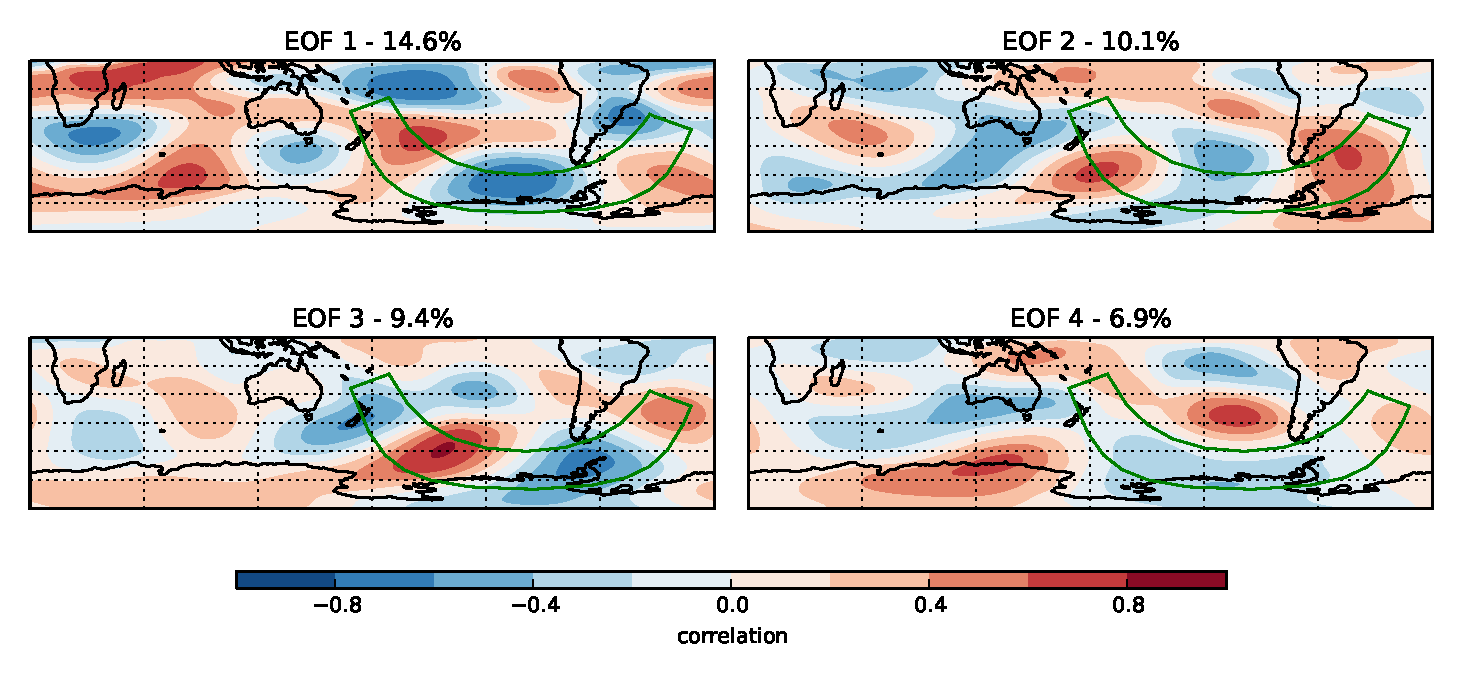
\includegraphics[width=1\columnwidth]{figures/psa/eof-sf_ERAInterim_500hPa_monthly_native-sh-zonal-anom.eps}
\caption[EOF analysis of the monthly 500 hPa zonal streamfunction anomaly]{\label{fig:eof}
Empirical Orthogonal Function (EOF) analysis of the monthly 500 hPa zonal streamfunction anomaly from the ERA-Interim reanalysis over the period 1979-2014. This is the most common method, variable and timescale used to investigate the PSA pattern and the data are presented as the correlation of the corresponding principal component with the original field. The second and third EOF modes are degenerate according to the \citet{North1982} rule of thumb, which means the sample eignenvectors (i.e. EOF-2 and EOF-3) represent a random mixture of the true eigenvectors. In this case, EOF-1 resembles the PSA-1 mode described in the literature, while EOF-3 resembles the PSA-2 mode. Different filtering, datasets, time periods and EOF methodologies influence the location and magnitude of the anomaly centres slightly, but the overall structure of the EOF-1 mode and the degenerate nature of EOF-2 and EOF-3 are a consistent feature. Green lines indicate the search region of interest defined in Section \ref{s:psa_id} (the `PSA sector') and the percentage of variance explained is indicated for each EOF mode.%
}
\end{center}
\end{figure}

It has been shown that the PSA pattern plays a role in blocking events \citep{Sinclair1997,Renwick1999}, South American rainfall variability \citep{Mo2001} and is also closely related to prominent regional features such as the ASL \citep{Turner2013}, Antarctic Dipole \citep{Yuan2001}, Antarctic Circumpolar Wave \citep{Christoph1998} and Southern Annular Mode \citep[SAM; e.g.][]{Ding2012}. While these are all important mid-to-high latitude impacts and relationships, in recent years the PSA pattern has been mentioned most frequently in the literature in relation to the rapid warming observed over West Antarctica and the Antarctic Peninsula \citep{Nicolas2014}. In particular, it has been suggested that seasonal trends in tropical Pacific SSTs may be responsible, via circulation trends resembling the PSA pattern, for winter (and to a lesser extent spring) surface warming in West Antarctica \citep{Ding2011} and autumn surface warming across the Antarctic Peninsula \citep{Ding2013}. The pattern has also been associated with declines in sea ice in the Amundsen and Bellingshausen Seas \citep{Schneider2012} and glacier retreat in the Amundsen Sea Embayment \citep{Steig2012}.

In identifying the PSA pattern as a possible contributor to these trends, the aforementioned studies looked through the lens of the variable/s of interest. For instance, \citet{Ding2011} performed a maximum covariance analysis to examine the relationship between central Pacific SSTs and the broader SH circulation (the 200hPa geopotential height). The second mode of that analysis revealed a circulation resembling the PSA pattern (and that brings warm air over West Antarctica), and atmospheric model runs forced with the associated central Pacific SSTs produced a PSA-like wave train. While this is certainly a valid research methodology, the result would be more robust if a climatology of PSA pattern activity also displayed trends consistent with warming in West Antarctica. This concept of teleconnection reversibility was recently invoked to question the relationship between Indian Ocean SSTs and heat waves in south-western Australia \citep{Boschat2016}.   

 
%========================

\section{The reproducibility crisis}

The rise of computational science has led to unprecedented opportunities in the weather and climate sciences. Ever more powerful computers enable experiments that would have been considered impossible only a decade ago, while new hardware technologies allow data collection in even the most inaccessible places. In order to analyse the vast quantities of data now available to them, modern practitioners -- most of whom are not computational experts -- use an increasingly diverse set of software tools and packages. Today's weather or climate scientist is far more likely to be found debugging code written in Python, MATLAB, Interactive Data Language (IDL), NCAR Command Language (NCL) or R, than to be poring over satellite images or releasing radiosondes. 

This computational revolution is not unique to the weather and climate sciences and has led to something of a reproducibility crisis in published research \citep[e.g.][]{Peng2011}. Most papers do not make the data and code underpinning key findings available, nor do they adequately specify the software packages and libraries used to execute that code. This means it is impossible to replicate and verify most of the computational results presented in journal articles today. By extension (and perhaps even more importantly), it is also impossible for readers to interrogate the data processing methodology. If a reader cannot find out which Python library was used in re-gridding a particular dataset, how can they build upon that re-gridding method and/or apply it in their own context? 

A movement within the computational science community has arisen in response to this crisis, calling for existing communication standards to be adapted to include the data and code associated with published findings \citep[e.g.][]{Stodden2014}. The movement has also been active in producing best practice recommendations to guide scientists and stakeholders \citep[e.g.][]{Prlic2012,Stodden2012a,Sandve2013,Stodden2014}, and similar calls and guidelines have appeared in numerous editorials and commentaries in recent years \citep[e.g.][]{Barnes2010,Merali2010,Ince2012}. In response to this sustained campaign, there has been a modest but perceptible reaction from funding agencies and academic journals. Agencies like the National Science Foundation now require dataset disclosure and encourage software availability, however this is not consistently enforced and compliance is largely left to the authors themselves \citep{Stodden2013}. A recent review of journal policies found a trend toward data and code availability, but overall the vast majority of journals have no data or code policy \citep{Stodden2013}. 

Similar to many other computational disciplines, in the weather and climate sciences progress on code availability is lagging behind data availability. The societies behind most of the major journals (American Meteorological Society, Royal Meteorological Society, American Geophysical Union and European Geosciences Union) all have official data policies \citep[e.g.][]{Mayernik2015}, however only two of the four indicate that code is included under their broad definition of data or metadata. Where code is included, statements regarding code availability consist of brief, vague suggestions that are not enforced by editors and reviewers. New journals such as \textit{Geoscientific Model Development} have arisen for documenting work where code/software is the primary output (e.g. the development of a new climate model), but little progress has been made in documenting the computational aspects of research where code is ancillary to the main focus (i.e. where the code is not of sufficient consequence to require a standalone paper devoted to its description). Given that much of the research conducted by weather and climate scientists is based on previously documented datasets and/or models (e.g. a paper might analyse a reanalysis dataset or the output from running a well-known atmospheric model forced with anomalous sea surface temperatures), ancillary code availability (as opposed to data availability or primary code availability) is the component of the reproducibility crisis common to essentially all research today.

While it is tempting to simply decry the slow response of journals and funding agencies in the face of this crisis, the reality is that examples of reproducible weather and climate research upon which to base new communication standards have only just begun to emerge. For instance, the Max Planck Institute for Meteorology (MPI-M) recently enacted a policy \citep{Stevens2015a} that requires all primary data (including ancillary code) to be archived, and papers adhering to that policy are now starting to be published \citep[e.g.][]{Stevens2015}. There are also a limited number of examples from other research disciplines, where highly motivated computational scientists have taken a variety of different approaches to publishing reproducible results \citep[e.g.][]{Hanigan2012,Ketcheson2012,Crooks2014,Bremges2015,Schmitt2015}. In order to set well informed communication standards, journals and funding agencies require many more examples of reproducible research, in addition to robust discussions on the practicalities of different approaches and how they might be implemented as formal standards.  


%========================

\section{Thesis outline}

This thesis presents a detailed climatological account of the major zonal asymmetries of the SH extratropical circulation. In order to overcome the shortcomings of current wave identification methods, new methods are devised that adapt data processing techniques more commonly used in meteorological and oceanographic research. The application of these new methods reveals many new insights into the characteristics of the ZW1, ZW3 and PSA pattern and their influence on regional climate variability and trends. The thesis also provides a practical solution to the reproducibility crisis in weather and climate research. Rather than adopt an approach that only works for the research at hand, a procedure for documenting the computational aspects of a research project was developed that reduces the barriers for researchers while also promoting good programming practices. It should provide a starting point for weather and climate scientists looking to publish reproducible research, and a detailed proposal is put forward outlining how the procedure might be adopted as a formal minimum standard by relevant academic journals.

The data, general data analysis techniques and computational procedures are outlined in Chapter \ref{c:methods}. The new wave identification methods and corresponding climatologies for the zonal waves and PSA pattern are then described in Chapters \ref{c:zw_climatology} and \ref{c:psa_climatology} respectively, while the practical solution to the reproducibility crisis is covered in Chapter \ref{c:reproducibility}. The major contributions of the thesis are summarised in Chapter \ref{c:conclusions}, along with a discussion of the associated limitations and directions for further research.